\documentclass[a4paper,11pt]{article}

\usepackage[margin=1.5cm]{geometry}
\usepackage{multicol}
\usepackage{listings}
\usepackage{xcolor}
\usepackage{tikz}
\usepackage[T1]{fontenc}

\usetikzlibrary{arrows.meta, positioning}

\lstset{
  basicstyle=\ttfamily\small,
  keywordstyle=\color{blue},
  commentstyle=\color{gray},
  breaklines=true
}

\begin{document}

\begin{center}
    {\Large \textbf{Formulario Git y GitHub}}\\
\end{center}

%%%%%%%%%%%%%%%%%%%%%%%%%%%%%%%%%%%%%%%%%%%%%%%%%%%%%%%%%%%%%%%

\section*{¿Qué es Git?}

Git es un sistema de:
\begin{itemize}
    \item Control de versiones
    \item Manejo de branches
    \item Trabajo colaborativo
    \item Historial de cambios
\end{itemize}

GitHub es una plataforma remota para repositorios Git.

%%%%%%%%%%%%%%%%%%%%%%%%%%%%%%%%%%%%%%%%%%%%%%%%%%%%%%%%%%%%%%%

\section*{Flujo básico}

\begin{lstlisting}
Working Directory
        |
        V
git add
        |
        V
Staging Area
        |
        V
git commit
        |
        V
Repositorio Local
        |
        V
git push
        |
        V
GitHub
\end{lstlisting}

%%%%%%%%%%%%%%%%%%%%%%%%%%%%%%%%%%%%%%%%%%%%%%%%%%%%%%%%%%%%%%%

\section*{Configuración inicial}

\begin{lstlisting}
git config --global user.name "Fulano"

git config --global user.email "mail@mail.com"
\end{lstlisting}

%%%%%%%%%%%%%%%%%%%%%%%%%%%%%%%%%%%%%%%%%%%%%%%%%%%%%%%%%%%%%%%

\section*{Inicializar repositorio}

\begin{lstlisting}
git init
\end{lstlisting}

%%%%%%%%%%%%%%%%%%%%%%%%%%%%%%%%%%%%%%%%%%%%%%%%%%%%%%%%%%%%%%%

\section*{Clonar repositorio}

\begin{lstlisting}
git clone URL
\end{lstlisting}

%%%%%%%%%%%%%%%%%%%%%%%%%%%%%%%%%%%%%%%%%%%%%%%%%%%%%%%%%%%%%%%

\section*{Estado}

\begin{lstlisting}
git status
\end{lstlisting}

%%%%%%%%%%%%%%%%%%%%%%%%%%%%%%%%%%%%%%%%%%%%%%%%%%%%%%%%%%%%%%%

\section*{Agregar archivos}

\begin{lstlisting}
git add file.cpp

git add .
\end{lstlisting}

%%%%%%%%%%%%%%%%%%%%%%%%%%%%%%%%%%%%%%%%%%%%%%%%%%%%%%%%%%%%%%%

\section*{Commit}

\begin{lstlisting}
git commit -m "Mensaje"
\end{lstlisting}

%%%%%%%%%%%%%%%%%%%%%%%%%%%%%%%%%%%%%%%%%%%%%%%%%%%%%%%%%%%%%%%

\section*{Push}

\begin{lstlisting}
git push origin main
\end{lstlisting}

%%%%%%%%%%%%%%%%%%%%%%%%%%%%%%%%%%%%%%%%%%%%%%%%%%%%%%%%%%%%%%%

\section*{Pull}

\begin{lstlisting}
git pull origin main
\end{lstlisting}

%%%%%%%%%%%%%%%%%%%%%%%%%%%%%%%%%%%%%%%%%%%%%%%%%%%%%%%%%%%%%%%

\section*{Branches}

Crear:
\begin{lstlisting}
git branch dev
\end{lstlisting}

Moverse:
\begin{lstlisting}
git checkout dev
\end{lstlisting}

Crear + mover:
\begin{lstlisting}
git checkout -b dev
\end{lstlisting}

%%%%%%%%%%%%%%%%%%%%%%%%%%%%%%%%%%%%%%%%%%%%%%%%%%%%%%%%%%%%%%%

\section*{Merge}

\begin{lstlisting}
git checkout main

git merge dev
\end{lstlisting}

Une historial de branches.

%%%%%%%%%%%%%%%%%%%%%%%%%%%%%%%%%%%%%%%%%%%%%%%%%%%%%%%%%%%%%%%

\section*{Rebase}

\begin{lstlisting}
git checkout dev

git rebase main
\end{lstlisting}

Reescribe historial para hacerlo lineal.

%%%%%%%%%%%%%%%%%%%%%%%%%%%%%%%%%%%%%%%%%%%%%%%%%%%%%%%%%%%%%%%

\section*{Fork}

Fork:
\begin{itemize}
    \item Copia remota de un repositorio
    \item Muy usado en Open Source
\end{itemize}

%%%%%%%%%%%%%%%%%%%%%%%%%%%%%%%%%%%%%%%%%%%%%%%%%%%%%%%%%%%%%%%

\section*{Fork Workflow}

\begin{center}

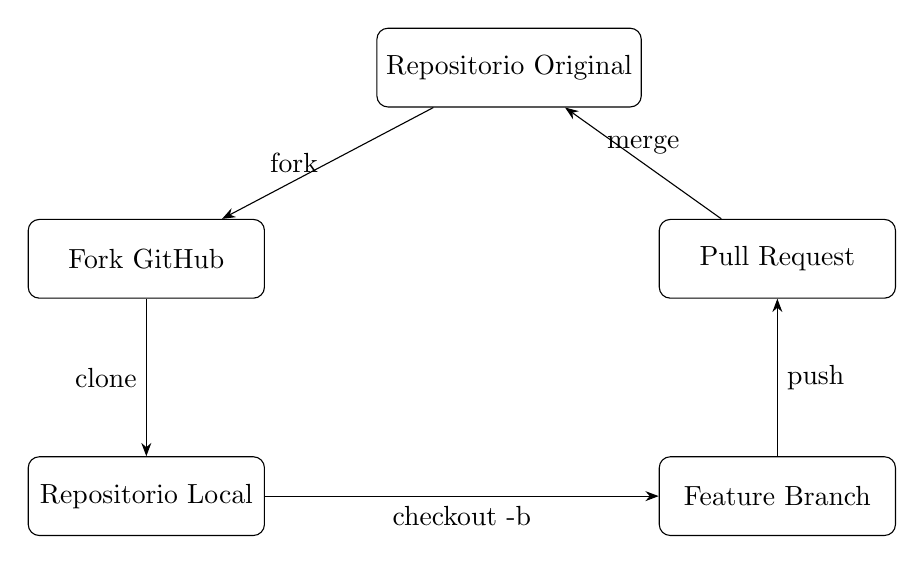
\begin{tikzpicture}[
node distance=2cm,
box/.style={
draw,
rounded corners,
minimum width=3cm,
minimum height=1cm
},
>=Stealth
]

\node[box] (upstream) {Repositorio Original};

\node[box, below left=of upstream] (fork)
{Fork GitHub};

\node[box, below=of fork] (local)
{Repositorio Local};

\node[box, right=5cm of local] (branch)
{Feature Branch};

\node[box, above=of branch] (pr)
{Pull Request};

\draw[->] (upstream) -- node[left]{fork} (fork);

\draw[->] (fork) -- node[left]{clone} (local);

\draw[->] (local) -- node[below]{checkout -b}
(branch);

\draw[->] (branch) -- node[right]{push} (pr);

\draw[->] (pr) -- node[above]{merge} (upstream);

\end{tikzpicture}

\end{center}

%%%%%%%%%%%%%%%%%%%%%%%%%%%%%%%%%%%%%%%%%%%%%%%%%%%%%%%%%%%%%%%

\section*{Historial}

\begin{lstlisting}
git log

git log --oneline

git log --graph
\end{lstlisting}

%%%%%%%%%%%%%%%%%%%%%%%%%%%%%%%%%%%%%%%%%%%%%%%%%%%%%%%%%%%%%%%

\section*{Reset}

\begin{lstlisting}
git reset HEAD~1
\end{lstlisting}

Tipos:
\begin{itemize}
    \item --soft
    \item --mixed
    \item --hard
\end{itemize}

%%%%%%%%%%%%%%%%%%%%%%%%%%%%%%%%%%%%%%%%%%%%%%%%%%%%%%%%%%%%%%%

\section*{Stash}

\begin{lstlisting}
git stash

git stash pop
\end{lstlisting}

Guardar cambios temporales.

%%%%%%%%%%%%%%%%%%%%%%%%%%%%%%%%%%%%%%%%%%%%%%%%%%%%%%%%%%%%%%%

\section*{Remote}

\begin{lstlisting}
git remote -v

git remote add origin URL
\end{lstlisting}

%%%%%%%%%%%%%%%%%%%%%%%%%%%%%%%%%%%%%%%%%%%%%%%%%%%%%%%%%%%%%%%

\section*{Tags}

\begin{lstlisting}
git tag v1.0

git push origin v1.0
\end{lstlisting}

%%%%%%%%%%%%%%%%%%%%%%%%%%%%%%%%%%%%%%%%%%%%%%%%%%%%%%%%%%%%%%%

\section*{Conflictos}

Ocurren cuando:
\begin{itemize}
    \item Dos branches modifican lo mismo
\end{itemize}

Resolver:
\begin{itemize}
    \item Editar archivos
    \item git add
    \item git commit
\end{itemize}

%%%%%%%%%%%%%%%%%%%%%%%%%%%%%%%%%%%%%%%%%%%%%%%%%%%%%%%%%%%%%%%

\section*{.gitignore}

\begin{lstlisting}
build/

*.o

*.exe

.env
\end{lstlisting}

%%%%%%%%%%%%%%%%%%%%%%%%%%%%%%%%%%%%%%%%%%%%%%%%%%%%%%%%%%%%%%%

\section*{GitHub Pull Request}

Flujo:
\begin{itemize}
    \item Crear branch
    \item Push
    \item Pull Request
    \item Review
    \item Merge
\end{itemize}

%%%%%%%%%%%%%%%%%%%%%%%%%%%%%%%%%%%%%%%%%%%%%%%%%%%%%%%%%%%%%%%

\section*{Cherry Pick}

\begin{lstlisting}
git cherry-pick HASH
\end{lstlisting}

Copiar commits específicos.

%%%%%%%%%%%%%%%%%%%%%%%%%%%%%%%%%%%%%%%%%%%%%%%%%%%%%%%%%%%%%%%

\section*{Submodules}

\begin{lstlisting}
git submodule add URL
\end{lstlisting}

Repositorio dentro de otro repositorio.

%%%%%%%%%%%%%%%%%%%%%%%%%%%%%%%%%%%%%%%%%%%%%%%%%%%%%%%%%%%%%%%

\section*{Git Flow simplificado}

\begin{lstlisting}
main
 |
 +---- develop
         |
         +---- feature/login
         |
         +---- feature/api
\end{lstlisting}

%%%%%%%%%%%%%%%%%%%%%%%%%%%%%%%%%%%%%%%%%%%%%%%%%%%%%%%%%%%%%%%

\section*{Comandos importantes}

\begin{center}
\begin{tabular}{| c | c |}
\hline
Comando & Descripción \\
\hline\hline
git status & Estado \\
\hline
git add & Staging \\
\hline
git commit & Commit \\
\hline
git push & Subir cambios \\
\hline
git pull & Descargar cambios \\
\hline
git branch & Branches \\
\hline
git checkout & Cambiar branch \\
\hline
git merge & Merge \\
\hline
git rebase & Rebase \\
\hline
git stash & Guardar temporalmente \\
\hline
\end{tabular}
\end{center}

%%%%%%%%%%%%%%%%%%%%%%%%%%%%%%%%%%%%%%%%%%%%%%%%%%%%%%%%%%%%%%%

\end{document}